\documentclass[tcc,capa]{texufpel}

\usepackage[utf8]{inputenc} % acentuacao
\usepackage{graphicx} % para inserir figuras
\usepackage[T1]{fontenc}
\usepackage{amsmath}

\hypersetup{
  hidelinks, % Remove coloração e caixas
  unicode=true,  %Permite acentuação no bookmark
  linktoc=all %Habilita link no nome e página do sumário
}

\unidade{Centro de Desenvolvimento Tecnológico}
\curso{Ciência da Computação}
\nomecurso{Bacharelado em Ciência da Computação}
\titulocurso{Bacharel em Ciência da Computação}

\unidadeeng{Technology Development Center}
\cursoeng{Computer Science}


\title{Um Blabla Blablabla com Aplicações em Blablabla}

\author{Aguiar}{Marilton Sanchotene de}
\advisor[Prof.~Dr.]{Aguiar}{Marilton Sanchotene de}
\coadvisor[Prof.~Dr.]{Aguiar}{Marilton Sanchotene de}
\collaborator[Prof.~Dr.]{Aguiar}{Marilton Sanchotene de}

%Palavras-chave em PT_BR
%use letras minúsculas seguidas por ;
%a última terminada por .
\keyword{palavrachave-um;}
\keyword{palavrachave-dois;}
\keyword{palavrachave-tres;}
\keyword{palavrachave-quatro.}

%Palavras-chave em EN_US
\keywordeng{keyword-one;}
\keywordeng{keyword-two;}
\keywordeng{keyword-three;}
\keywordeng{keyword-four.}

\usepackage{tikz}
\usetikzlibrary{arrows.meta, shapes, positioning}

\begin{document}

%\renewcommand{\advisorname}{Orientadora}      %descomente caso tenhas orientadora
%\renewcommand{\coadvisorname}{Coorientadora}   %descomente caso tenhas coorientadora

\maketitle 

\sloppy

\fichacatalografica

%\folhadeaprovacao

%Composição da Banca Examinadora
\begin{aprovacao}{30 de fevereiro de 2019} %data da banca por extenso
\noindent Prof. Dr. Marilton Sanchotene de Aguiar (orientador)\\
Doutor em Computação pela Universidade Federal do Rio Grande do Sul.\\[1cm]

\noindent Prof. Dr. Paulo Roberto Ferreira Jr.\\
Doutor em Computação pela Universidade Federal do Rio Grande do Sul.\\[1cm]

\noindent Prof. Dr. Ricardo Matsumura Araujo\\
Doutor em Computação pela Universidade Federal do Rio Grande do Sul.\\[1cm]

\noindent Prof. Dr. Luciano da Silva Pinto\\
Doutor em Biotecnologia pela Universidade Federal de Pelotas.
\end{aprovacao}

%Opcional
\begin{dedicatoria}
 Dedico\ldots 
\end{dedicatoria}

%Opcional
\begin{agradecimentos}
 Agradeço\ldots 
\end{agradecimentos}

%Opcional
\begin{epigrafe}
 Só sei que nada sei.\\
 {\sc --- Sócrates}
\end{epigrafe}

%Resumo em Portugues (no maximo 500 palavras)
\begin{abstract}
\end{abstract}

%Resumo em Inglês (no maximo 500 palavras)
\begin{englishabstract}{Titulo do Trabalho em Ingles}
\end{englishabstract}

%Lista de Figuras
\listoffigures

%Lista de Tabelas
\listoftables

% Lista de abreviaturas e siglas
\begin{listofabbrv}{LLMDA}%coloque aqui a maior sigla para ajustar a distância
    \item[ASL] American Sign Language
    \item[SLR] Sign Language Recognition
    \item[SLT] Sign Language Translation
    \item[LSA-T] Lengua de Señas Argentina - Traduction
    \item[LSFB] Langue des Signes de Belgique Francophone
    \item[ISL] Indian Sign Language
    \item[GSL] Greek Sign Language
    \item[CVPR] Conference on Computer Vision and Pattern Recognition
    \item[ICLR] International Conference on Learning Representations
    \item[IJCNN] International Joint Conference on Neural Networks
    \item[FG] IEEE International Conference on Automatic Face and Gesture Recognition
    \item[WACV] IEEE Winter Conference on Applications of Computer Vision
    \item[ACL] Association for Computational Linguistics
    \item[EMNLP] Conference on Empirical Methods in Natural Language Processing
    \item[LREC] Language Resources and Evaluation Conference
    \item[BLEU] Bilingual Evaluation Understudy
    \item[chrF] Character n-gram F-score
    \item[SBERT] Sentence-BERT
    \item[BERT] Bidirectional Encoder Representations from Transformers
    \item[BT] Back-Translation
    \item[LLM] Large Language Model
    \item[LLMDA] Large Language Model Data Augmentation
    \item[RGB-D] Red-Green-Blue + Depth (profundidade)
\end{listofabbrv}


%Sumario
\tableofcontents

\chapter{Introdução}

As línguas de sinais constituem sistemas linguísticos plenos, com gramática e léxico próprios, distintos tanto da língua oral quanto de sua forma escrita. Em diversos países, a distância entre essas modalidades, aliada a barreiras históricas de acesso educacional, contribui para que parte dos estudantes surdos conclua a educação básica com proficiência leitora aquém do esperado para o currículo regular \cite{Traxler2000}. Nesse cenário, sistemas de tradução automática de língua de sinais para texto (SLT) surgem como tecnologia de mediação: aproximam a comunidade surda de conteúdos escritos e ampliam as possibilidades de interação com ouvintes em ambientes acadêmicos, profissionais e de serviços.

Do ponto de vista computacional, a SLT permanece desafiadora. O sinal transmite significado de forma simultânea por mãos, face e corpo, com forte coarticulação e variação inter/intra-sinalizador; além disso, há escassez de corpora paralelos com alinhamento temporal consistente e evidente sensibilidade a mudanças de domínio (\emph{domain shift}) entre línguas, cenários de captura e protocolos de anotação. A literatura recente modela SLT como um problema sequência–para–sequência com atenção e discute escolhas de representação que vão do vídeo bruto a sequências cinemáticas de pontos-chave (\emph{keypoints}) \cite{Camgoz2018NeuralSLT,Koller2020SurveySLR}. Enquanto o vídeo preserva textura e pistas não manuais, os \emph{keypoints} condensam a dinâmica articulatória essencial e tendem a ser mais portáveis entre cenários, sobretudo quando extraídos por pipelines estáveis \cite{Lugaresi2019MediaPipe,MediaPipeHolisticDocs}.

Neste trabalho, formulamos a seguinte hipótese: é possível aumentar a \emph{generalização} em SLT treinando um único modelo orientado a \emph{keypoints} sobre múltiplas línguas e múltiplos corpora, apoiado por \emph{data augmentation} textual e cinemático cuidadosamente controlado. Para testá-la, adotamos o \emph{Signformer} \cite{Yang2024Signformer} como arquitetura base, unificamos diferentes bases em um manifesto comum e investigamos estratégias complementares de aumento de dados (paráfrases/retrotradução no texto e perturbações plausíveis nas poses) com o objetivo explícito de robustez fora do domínio, entre línguas, sinalizadores e condições de gravação.

A proposta avança em três frentes integradas. Primeiro, realizamos a integração e padronização de corpora heterogêneos de SLT, normalizando texto e \emph{keypoints} em um esquema único que viabiliza experimentação comparável. Segundo, treinamos um único \emph{Signformer} multilíngue e \emph{multi-corpora}, explorando a representação \emph{gloss-free} para reduzir variância espúria e aumentar portabilidade. Terceiro, avaliamos o papel do \emph{augmentation} na melhoria da capacidade de generalização com protocolos que incluem testes \emph{cross-domain} e \emph{signer-held-out}, reportando métricas lexicais e semânticas alinhadas à prática da área.

Em síntese, este estudo busca contribuir para uma linha de SLT mais pragmática e escalável: menos dependente de anotações intermediárias onerosas, mais consciente das fontes de variação que se impõem na prática, e orientada por um desenho experimental que privilegia generalização. A dissertação está organizada da seguinte forma: o Capítulo~2 apresenta o referencial teórico essencial e os trabalhos correlatos; o Capítulo~3 descreve a metodologia, os dados e as estratégias de \emph{augmentation}; o Capítulo~4 discute os resultados obtidos; e o Capítulo~5 reúne as conclusões e perspectivas futuras.

\chapter{Referencial Teórico}

A Tradução Automática de Língua de Sinais (SLT) pode ser entendida como um mapeamento probabilístico entre uma sequência multimodal de sinais visuais e uma sequência textual. Esse mapeamento repousa em três pilares: propriedades linguísticas das línguas sinalizadas, nas quais informações manuais e não manuais se combinam de forma simultânea e coarticulada;  escolhas de \emph{representação} do sinal, preservando aparência ou abstraindo para trajetórias cinemáticas; e  modelos sequenciais que estabelecem alinhamentos (explícitos ou implícitos) entre segmentos temporais e unidades linguísticas. Camgoz et al.\ descrevem a SLT como um problema seq2seq com atenção que aprende alinhamentos flexíveis diretamente de dados visuais e textuais, enquanto Koller et al.\ apresentam, em sua revisão, a perspectiva de que simultaneidade, coarticulação e variação idiossincrática impõem vieses indutivos específicos às arquiteturas de modelagem. Em termos mais abstratos, a SLT projeta uma \textbf{variedade visual-linguística} de alta dimensão para um espaço simbólico discretizado, preservando \emph{composicionalidade} e \emph{equivalência proposicional} apesar da iconicidade e da heterogeneidade de realizadores. \cite{Camgoz2018NeuralSLT,Koller2020SurveySLR}

\section{Línguas de sinais: camadas informativas e simultaneidade}
Línguas de sinais codificam significado por meio de múltiplos articuladores, mãos (configuração, orientação, trajetória), componentes faciais (expressões, movimentos oculares), cabeça e tronco (inclinação, postura) e marcadores não manuais (labialização). Diferentemente de cadeias acústicas estritamente lineares, essas camadas são \textbf{simultâneas} e exibem \textbf{coarticulação}: um segmento influencia o seguinte, e traços não manuais frequentemente se estendem por janelas temporais mais longas do que gestos manuais. Koller et al.\ enfatizam que essa simultaneidade desfaz a suposição de alinhamento 1:1 entre porções do sinal e palavras, colocando a atenção como mecanismo natural para lidar com dependências de longo alcance e espalhamento prosódico. Nesse quadro, prosódia não manual veicula funções gramaticais (escopo de negação/interrogação, foco) e processos morfológicos simultâneos (classificadores, modificações espaciais) desafiam modelagens puramente concatenativas, o que explica a centralidade de representações e modelos capazes de acomodar sobreposição temporal e variação inter/intra-sinalizador. \cite{Koller2020SurveySLR}

\section{Formulação probabilística do mapeamento}
Dado um enunciado sinalizado $\mathbf{x}_{1:T}$ e um texto alvo $\mathbf{y}_{1:U}$,
\[
p(\mathbf{y}\mid\mathbf{x}) \;=\; \prod_{u=1}^{U} p\!\left(y_u \mid y_{<u},\, \mathbf{H}\right),
\qquad
\mathbf{H}=\mathrm{Encoder}(\mathbf{x}_{1:T}).
\]
Aqui, $\mathbf{H}$ resume a sequência de sinais, e o próximo token textual depende da história já gerada e de um \textbf{resumo atencional} da entrada. Bahdanau et al.\ introduzem a atenção como “aprender a alinhar e traduzir” via pesos que distribuem \emph{responsabilidade explicativa} de cada saída sobre múltiplas posições de entrada; Vaswani et al.\ substituem recorrência por \emph{autoatenção}, argumentando que dependências longas podem ser modeladas mais diretamente por conexões globais sobre a sequência. Camgoz et al.\ exploram essa visão no contexto de SLT, destacando que o alinhamento necessário é frequentemente \emph{não monotônico} por conta da coarticulação e das camadas não manuais, o que reforça a utilidade de mecanismos atencionais como variáveis latentes de correspondência. \cite{Bahdanau2015NMT,Vaswani2017Attention,Camgoz2018NeuralSLT}

\section{Representações de entrada}

\paragraph{Vídeo bruto.}
Tratar o sinal como sequência de quadros (RGB, profundidade, \textit{multiview}) preserva \textbf{pistas não manuais} e \textbf{textura}. Dosovitskiy et al.\ argumentam que a \emph{autoatenção} aplicada diretamente a \emph{patches} de imagem (ViT) permite modelar interações de longo alcance na dimensão espacial, o que, combinado a módulos temporais, fornece um caminho conceitual para capturar regularidades visuais relevantes. Duarte et al.\ apresentam o \textit{How2Sign} e destacam que variações de ponto de vista e profundidade capturam melhor a articulação espacial e os marcadores não manuais, reforçando a ideia de que representações visuais ricas suportam recuperabilidade dos traços linguísticos, ainda que aumentem a exposição a fatores espúrios. \cite{Dosovitskiy2021ViT,Duarte_2021_CVPR}

\paragraph{Representação cinemática por \emph{keypoints}.}
Ao descrever cada quadro por \emph{landmarks} 2D/3D de corpo, mãos e face,
\[
\mathbf{k}_t = \big[\,(x_j^{(t)},y_j^{(t)}[,z_j^{(t)}])\,\big]_{j\in\mathcal{J}}\in\mathbb{R}^{d},\quad d=|\mathcal{J}|\times\{2,3\},
\]
abstrai-se aparência e concentra-se a informação em \textbf{geometria} e \textbf{movimento}. Lugaresi et al.\ apresentam a família \emph{MediaPipe} como arcabouço de extração leve e consistente de \emph{landmarks}, e a documentação do \emph{MediaPipe Holistic} explicita a integração de corpo, mãos e face em um único grafo esquelético. Kim et al.\ sustentam que \emph{keypoints} reduzem dimensionalidade e introduzem invariâncias a transformações rígidas, enquanto Yang et al.\ propõem arquiteturas específicas (p.\,ex., \emph{Signformer}) para explorar dependências espaço-temporais sobre trajetórias articulares; em ambos os casos, o argumento comum é que a \emph{desvisualização} aproxima o espaço observável do espaço articulatório, com possível perda de micro–pistas de aparência relevantes. \cite{Lugaresi2019MediaPipe,MediaPipeHolisticDocs,Kim2022KeypointSLT,Yang2024Signformer}

\section{Arquiteturas: alinhamento explícito vs.\ implícito}
Na abordagem \textbf{em cascata}, introduz-se uma camada intermediária discreta (como \emph{glossas}) que torna o alinhamento \textbf{explícito}. Koller et al.\ pontuam que esta mediação simbólica impõe um viés de \emph{discretude} que pode facilitar aprendizagem e análise quando há anotações temporais confiáveis, ao custo de dependência de rótulos e de um duto mais rígido. Nas formulações \textbf{\emph{end-to-end}}, por sua vez, Camgoz et al.\ argumentam que o alinhamento é \textbf{latente} e a correspondência contínua entrada–texto é aprendida via atenção, o que torna o sistema mais fiel à simultaneidade natural das línguas de sinais e menos dependente de segmentações a priori. Em ambos os relatos, a questão de fundo é a \textbf{identificabilidade} do alinhamento sob dados finitos e o balanço entre viés indutivo e flexibilidade estatística. \cite{Koller2020SurveySLR,Camgoz2018NeuralSLT} 

\section{Benchmarks e o conceito de \emph{domain shift}}
Benchmarks variam quanto à língua, registro e captura, definindo tarefas e protocolos comparáveis. Forster et al.\ descrevem a família PHOENIX como um marco para avaliação de DGS em contexto de telejornal, enquanto Duarte et al.\ apresentam um cenário multimodal e multivisão para ASL; ambos os casos ilustram que “bom desempenho” pode estar condicionado ao domínio de coleta. Fink et al.\ e a revisão de Koller et al.\ chamam atenção para o \textbf{\emph{domain shift}}, discrepâncias entre treino e teste, que pode se manifestar como \emph{covariate shift} (mudança nos observáveis), \emph{label/target shift} (mudança na distribuição textual) ou \emph{concept shift} (mudança na relação entrada–saída). O consenso entre esses autores é que generalização requer representações que preservem invariantes linguísticos e protocolos de avaliação conscientes de cruzamentos de língua, cenário e sensor. \cite{forster2014extensions,Duarte_2021_CVPR,Fink2021,Koller2020SurveySLR}

\section{Padronização \emph{multi-corpora} e manifesto de dados}
Combinar corpora heterogêneos exige resolver \textbf{compatibilização semântica}: normalização textual (Unicode, caixa, pontuação), metadados (códigos ISO, \emph{splits}, identidades de sinalizadores, FPS), ordenações de \emph{keypoints} e critérios de qualidade (fração de marcos válidos). O repositório comunitário de SLT e a documentação \emph{MediaPipe} convergem na defesa de um \textbf{manifesto} tabular que explicite proveniência, esquema e critérios de validade, servindo como contrato reproduzível entre dados e modelos. Sennrich et al.\ e Kudo discutem tokenização em subpalavras como mecanismo para tornar a distribuição textual mais \emph{estimável} sob dados finitos, argumento que se encaixa naturalmente em cenários multi\-corpóras/multilíngues. \cite{slt_datasets_repo,Lugaresi2019MediaPipe,MediaPipeHolisticDocs,Sennrich2016BPE,Kudo2018SentencePiece}

\paragraph{Tokenização em subpalavras.}
Sennrich et al.\ introduzem BPE como fusão iterativa de pares frequentes para construir um vocabulário compacto que reduz \emph{OOV} e suaviza cauda longa; Kudo descreve o SentencePiece como treinamento direto em texto cru de modelos BPE/unigram, dispensando segmentadores externos e tratando tokens como variáveis latentes com probabilidades. Em ambos os relatos, a tese central é equilibrar \textbf{expressividade} lexical e \textbf{eficiência} estatística, com a decisão de compartilhar vocabulários entre corpora/línguas interpretada como um grau de \textbf{acoplamento} entre domínios. \cite{Sennrich2016BPE,Kudo2018SentencePiece}

\section{Aumento textual e preservação semântica}
Sennrich et al.\ propõem \textbf{retrotradução} como forma de gerar pares sintéticos a partir de alvos monolíngues; Edunov et al.\ mostram que a técnica escala com ganhos robustos em NMT; Wieting e Gimpel introduzem corpora de \textbf{paráfrases} em larga escala (ParaNMT) para diversificar a forma mantendo sentido. No contexto de SLT, Zhou et al.\ descrevem a \emph{Sign Back-Translation} como adaptação do princípio ao domínio sinalizado; trabalhos recentes (\cite{Ding2024LLMDA,ChatGPTDA2023,Oh2023LLMDA}) discutem LLMs como geradores controláveis de variantes sob restrições de fidelidade semântica. Em todos os casos, o fio comum é tratar aumento como \textbf{amostragem condicionada ao significado}, ampliando a superfície linguística sem alterar proposições. \cite{Sennrich2016BT,Edunov2018BTScale,Wieting2018ParaNMT,Zhou2021SignBT,Ding2024LLMDA,ChatGPTDA2023,Oh2023LLMDA}

\paragraph{Critérios semântico–superficiais.}
Reimers e Gurevych apresentam o \textbf{SBERT} como forma de obter \emph{embeddings} sentenciais que preservam semântica em espaço vetorial, possibilitando medir a proximidade por cosseno; Popović propõe \textbf{chrF}/\textbf{chrF++} como métricas de sobreposição em nível de caractere/palavra. A prática recomendada na literatura é aceitar uma variante $\tilde{y}$ quando ela maximiza similaridade semântica e controla proximidade superficial, refletindo a intuição de que diversidade útil exige preservar \textbf{equivalência proposicional} sem colapsar para cópia. \cite{Reimers2019SBERT,Popovic2015chrF,Popovic2017chrFpp}

\section{Aumentos cinemáticos e plausibilidade}
No espaço de \emph{keypoints}, trabalhos como os de Kocabas et al.\ e Springer et al.\ discutem apagamentos e oclusões sintéticas como forma de robustificar modelos a falhas de \emph{tracking}; Gong et al.\ apresentam o \emph{PoseAug} como gerador diferenciável de variações sob restrições geométricas; estudos recentes em WACV 2024 reforçam a necessidade de \textbf{aumentos realistas} que respeitem antropometria e dinâmica plausível. A literatura converge em quantificar \textbf{plausibilidade cinemática} por consistência de comprimentos de “ossos” no grafo esquelético e por suavidade temporal de velocidades e acelerações, evitando trajetórias fisicamente incoerentes que confundiriam a inferência. Formalmente,
\[
\phi(\mathbf{K})=\frac{1}{|\mathcal{B}|\,T}\sum_{t=1}^T\sum_{(p,q)\in\mathcal{B}}
\left|\,\|\hat{\mathbf{p}}_t-\hat{\mathbf{q}}_t\|_2 - \overline{\ell}_{pq}\,\right|,\quad \text{aceita-se se } \phi(\mathbf{K})\le\tau.
\]
\cite{WACV2020KeypointDropout,Springer2021OcclusionDropout,Gong2021PoseAug,WACV2024RealisticSkelAug,MediaPipeHolisticDocs}

\section{Avaliação: métricas lexicais e semânticas}
Post argumenta pela padronização de \textbf{sacreBLEU} para garantir comparabilidade entre estudos que reportam \textsc{BLEU}, cuja essência é combinar precisões de \emph{n}-gramas com penalização de brevidade; Popović propõe \textbf{chrF}/\textbf{chrF++} para capturar variação morfológica e escolhas lexicais em nível de caractere/palavra; Zhang et al.\ introduzem o \textbf{BERTScore} para avaliar \textbf{equivalência semântica} via similaridade de \emph{embeddings} contextualizados. A leitura convergente desses autores é que SLT requer um \emph{painel} de métricas: medidas lexicais estimam sobreposição de superfície, enquanto medidas baseadas em \emph{embeddings} aproximam similaridade de significado, de modo complementar. Em notação,
\[
\textsc{BLEU} = \mathrm{BP}\cdot \exp\!\bigg(\sum_{n=1}^{N} w_n \log p_n\bigg),\ \ 
\mathrm{BP}=\min\!\left(1, e^{1-\frac{r}{c}}\right),\quad
P=\frac{1}{|Y|}\sum_{j}\max_i s_{ij},\ 
R=\frac{1}{|X|}\sum_{i}\max_j s_{ij},\ 
F_1=\frac{2PR}{P+R}.
\]
\cite{Post2018SacreBLEU,Popovic2015chrF,Popovic2017chrFpp,Zhang2019BERTScore}

\chapter{Trabalhos Correlatos}

A tradução automática de Língua de Sinais (SLT) tem avançado em duas frentes que, por muito tempo, caminharam separadas:\emph{pipelines} em cascata (reconhecimento contínuo $\rightarrow$ glossas $\rightarrow$ texto) e  modelos \emph{end-to-end} que mapeiam diretamente vídeo para sentença. Camgoz et al.~\cite{Camgoz2018NeuralSLT} consolidaram a segunda vertente ao mostrar que atenção e modelagem seq2seq lidam com dependências temporais longas e a variação de velocidade/coarticulação típica da língua de sinais. Em paralelo, levantamentos como Koller~\cite{Koller2020SurveySLR} sistematizaram lições do reconhecimento contínuo (CSLR), destacando tanto o valor das glossas como supervisão quanto os limites desse recurso diante do custo de anotação e da heterogeneidade entre corpora.

No que diz respeito às \textit{entradas}, há um eixo que aposta na riqueza do \emph{vídeo bruto} (RGB, profundidade, multiview) e outro que aposta na compressão \emph{cinemática} por \emph{keypoints} (corpo, mãos e face). O \textit{How2Sign}~\cite{Duarte_2021_CVPR} impulsionou o primeiro eixo ao oferecer um recurso multiview e com profundidade para ASL, permitindo arquiteturas CNN/ViT + Transformer com maior cobertura dos sinais não manuais. Por outro lado, trabalhos recentes mostram que sequências de marcos normalizados podem ser suficientes para SLT, com ganhos de portabilidade e custo computacional~\cite{Kim2022KeypointSLT}. Nessa linha, o \emph{Signformer}~\cite{Yang2024Signformer} propõe atenção temporal diretamente sobre \emph{keypoints} extraídos (por exemplo, via MediaPipe~\cite{Lugaresi2019MediaPipe,MediaPipeHolisticDocs}), explorando invariâncias a fundo, iluminação e enquadramento e facilitando a análise mais interpretável dos focos de atenção.

Os \emph{benchmarks} que sustentam a área evoluíram de cenários de estúdio para contextos mais realistas e diversos. O \textit{RWTH-PHOENIX-Weather 2014} foi ampliado e se tornou referência para DGS$\rightarrow$alemão~\cite{forster2014extensions,koller2015continuous}; o \textit{split} de tradução (\textit{2014T}) foi posteriormente introduzido por Camgoz et al.~\cite{Camgoz2018NeuralSLT}. O \textit{LSA-T} ampliou a cobertura para LSA$\rightarrow$espanhol em notícias~\cite{DalBianco:2022:LSAT}; o \textit{How2Sign} trouxe multiview e profundidade para ASL~\cite{Duarte_2021_CVPR}; o \textit{LSFB-CONT} organizou narrativas controladas para LSFB$\rightarrow$francês~\cite{Fink2021}; o \textit{ISLTranslate} focou em ISL$\rightarrow$inglês, com material de domínio público e conteúdo educacional~\cite{joshi-etal-2023-isltranslate,ISLTranslateRepo}; e o \textit{GSL Continuous} cobriu GSL$\rightarrow$grego com gravações contínuas~\cite{GSL2020}. Apesar desse progresso, persiste um desafio recorrente: modelos treinados em um único corpus tendem a sofrer com \emph{domain shift} quando mudamos de língua, cenário de captura ou protocolo de anotação.

Para mitigar a escassez de paralelos e reduzir a esparsidade lexical, a comunidade de MT recorre há anos à retrotradução~\cite{Sennrich2016BT,Edunov2018BTScale} e à geração de paráfrases em larga escala~\cite{Wieting2018ParaNMT}; parte desse repertório também mostrou efeitos positivos em SLT, como a \emph{Sign Back-Translation}~\cite{Zhou2021SignBT}. Mais recentemente, LLMs vêm sendo empregados para produzir dados sintéticos com maior controle semântico e diversidade superficial~\cite{Ding2024LLMDA,ChatGPTDA2023,Oh2023LLMDA}. Em paralelo, do lado dos \emph{keypoints}, surgiram estratégias de \emph{augmentation} voltadas à robustez a oclusões e ruído de rastreamento, como \emph{keypoint dropout}, \emph{time warping} e \emph{auto-augmentation} geométrica (\emph{PoseAug}), que vêm se mostrando promissoras em tarefas baseadas em esqueleto~\cite{WACV2020KeypointDropout,Springer2021OcclusionDropout,Gong2021PoseAug,WACV2024RealisticSkelAug}.

À luz desse panorama, este trabalho se posiciona em três pontos de contato com a literatura:adota uma representação \emph{gloss-free} por \emph{keypoints} no espírito do \emph{Signformer}~\cite{Yang2024Signformer,Kim2022KeypointSLT}, visando reduzir variância espúria e melhorar a interpretabilidade;  opera sobre \emph{múltiplos} corpora de línguas e domínios distintos (PHOENIX-2014/2014T, LSA-T, How2Sign, LSFB-CONT, ISLTranslate, GSL)~\cite{forster2014extensions,koller2015continuous,Camgoz2018NeuralSLT,DalBianco:2022:LSAT,Duarte_2021_CVPR,Fink2021,joshi-etal-2023-isltranslate,GSL2020}, enfrentando explicitamente o \emph{domain shift} que a literatura frequentemente evita ao avaliar um corpus por vez; e  explora aumento textual com LLMs (paráfrases e retrotradução) combinado a \emph{augmentations} de pose com checagens cinemáticas, buscando ganhos de generalização sem sacrificar plausibilidade linguística e articulatória~\cite{Sennrich2016BT,Edunov2018BTScale,Wieting2018ParaNMT,Ding2024LLMDA,ChatGPTDA2023,Oh2023LLMDA,WACV2020KeypointDropout,Springer2021OcclusionDropout,Gong2021PoseAug,WACV2024RealisticSkelAug}.

\chapter{Metodologia}

\section{Bases de Dados Utilizadas}

No presente trabalho, emprega-se um conjunto abrangente e heterogêneo de corpora voltados à tradução automática de Língua de Sinais, contemplando diferentes idiomas, domínios, formatos de mídia e níveis de anotação. Com o intuito de assegurar a comparabilidade dos resultados e maximizar a capacidade de generalização dos modelos, todas as bases de dados foram previamente integradas em um repositório unificado, por meio de procedimentos sistemáticos de padronização de formatos, normalização textual e harmonização de metadados. A seguir, descrevem-se individualmente cada um desses conjuntos de dados, destacando suas principais características e especificidades.

\subsection{RWTH-PHOENIX-Weather 2014 T}

O \textit{RWTH-PHOENIX-Weather 2014 T} foi desenvolvido pelo grupo \textit{Human Language Technology and Pattern Recognition} da RWTH Aachen University, com o objetivo de estabelecer um benchmark robusto para tarefas de reconhecimento contínuo e tradução automática da Língua de Sinais Alemã (DGS) para o alemão escrito \cite{koller2015continuous,forster2014extensions}. O corpus deriva de transmissões autênticas de previsão do tempo do canal público alemão \textit{Phoenix}, gravadas entre 2009 e 2011, preservando a naturalidade e o contexto de uso real da língua.

\textbf{Composição} (fonte: RWTH) \cite{koller2015continuous,forster2014extensions}:
\begin{itemize}
 \item \textbf{Domínio}: transmissões televisivas de previsão do tempo, com intérpretes profissionais enquadrados em plano médio fixo, vestimenta predominantemente escura e fundo neutro, garantindo contraste e consistência visual.
 \item \textbf{Formato dos vídeos}: resolução de 210 × 260 px, taxa de 25 quadros por segundo (\textit{FPS}); vídeos codificados em MPEG-4.
 \item \textbf{Dados anotados}: corpus com 2\,887 pares de sentenças (glossas e texto em alemão), alinhados temporalmente ao nível de palavra sinalizada. Dividido em 2\,612 exemplos para treino, 250 para validação e 228 para teste.
 \item \textbf{Vocabulário}: 768 glossas distintas na DGS e 1\,389 palavras únicas no alemão escrito. A taxa de \emph{singletons} é de 32,4\% no conjunto de glossas e 36,4\% no texto.
 \item \textbf{Participantes}: 7 intérpretes surdos ou ouvintes fluentes, predominantemente destros, garantindo variação natural de estilo e velocidade de sinalização.
 \item \textbf{Anotações complementares}: arquivos XML contendo alinhamento temporal das glossas e transcrições completas; segmentação respeitando o início e o fim de cada sentença.
\end{itemize}

\subsection{LSA-T}

O dataset \textit{LSA-T} (Lengua de Señas Argentina - Traducción) foi desenvolvido por Dal Bianco et al., sendo o primeiro corpus contínuo de tradução da Língua de Sinais Argentina (LSA) para o espanhol escrito \cite{DalBianco:2022:LSAT}. O material foi extraído do canal de notícias CN Sordos no YouTube, englobando vídeos com diversos sinalizadores, cenários, iluminação e sotaques, atributos que o tornam particularmente robusto para avaliação de modelos em contextos reais.

\textbf{Composição} (fonte: repositório oficial e papers) \cite{DalBianco:2022:LSAT}:
\begin{itemize}
 \item \textbf{Domínio}: vídeos de notícias em LSA com legendas em espanhol; diversidade visual e contextual significativa.
 \item \textbf{Formato dos vídeos}: Full HD (1920 × 1080px), 30 quadros por segundo (FPS), codificados em formato MP4.
 \item \textbf{Dados anotados}: 14\,880 segmentos de vídeo, cada um contendo uma frase com legendas correspondentes e coordenadas de pose por Mediapipe.
 \item \textbf{Vocabulário}: aproximadamente 14\,239 palavras únicas; cerca de 50\% de \emph{singletons}, indicando grande variação lexical e desafio para modelos tradicionais.
 \item \textbf{Participantes}: 103 sinalizadores (mostly guest signers), com diversidade de gênero e aparições esporádicas, mantendo equilíbrio e autenticidade.
 \item \textbf{Anotações complementares}: keypoints (pose) extraídos de cada vídeo; identificação do sinalizador ativo em casos com múltiplas pessoas em cena.
\end{itemize}

\subsection{How2Sign}

O corpus \textit{How2Sign} foi apresentado por Duarte et al. com o objetivo de criar o maior dataset contínuo, multimodal e multiview da Língua de Sinais Americana (ASL), voltado à tradução e produção automática de sinais \cite{Duarte_2021_CVPR}. Ele consiste em vídeos “como fazer” em inglês, interpretados em ASL, com anotação extensa e variada.

\textbf{Composição} (fontes: Duarte et al., CVPR 2021) \cite{Duarte_2021_CVPR}:
\begin{itemize}
 \item \textbf{Volume de dados}: mais de 80 horas de vídeo multiview (RGB frontal, lateral e profundidade).
 \item \textbf{Subset Panoptic}: cerca de 3 horas registradas em estúdio especializado, permitindo estimativas de pose 3D de alta fidelidade.
 \item \textbf{Segmentos anotados}: aproximadamente 35 191 sentenças alinhadas com transcrições em inglês e glossas ASL.
 \item \textbf{Duração média por segmento}: cerca de 5,4 segundos (~162 quadros a 30 FPS).
 \item \textbf{Vocabulário}: cerca de 16 000 palavras únicas em inglês, com diversidade temática ampla.
 \item \textbf{Participantes}: 11 sinaladores (5 ouvintes, 4 surdos, 2 com audição parcial); um test-set inclui 26 vídeos de um sinalador não presente no treinamento, para avaliar generalização.
\end{itemize}

\subsection{LSFB-CONT}

O \textit{LSFB-CONT} (Langue des Signes de Belgique Francophone – Continuous) foi criado pelo Laboratoire de Traitement de la Parole et de la Langue (LTPL) da Universidade de Namur, em colaboração com o Serviço de Interpretação para Surdos da Bélgica Francófona \cite{Fink2021}. O corpus foi concebido para pesquisas em reconhecimento contínuo e tradução da LSFB para o francês escrito, representando um recurso de referência para estudos de modelagem linguística e visão computacional.

\textbf{Composição} (fonte: Fink et al., 2021) \cite{Fink2021}:
\begin{itemize}
 \item \textbf{Domínio}: produções narrativas e descritivas de sinaladores nativos de LSFB, abrangendo histórias pessoais, descrições de imagens estáticas e resumos de curtas-metragens. As gravações foram realizadas em ambiente controlado, com plano médio fixo, fundo neutro e iluminação uniforme.
 \item \textbf{Formato dos vídeos}: resolução de 720 × 576 px, taxa de 50 quadros por segundo (\textit{FPS}); codificação MPEG-2, áudio sincronizado para referência de legendas.
 \item \textbf{Volume de dados}: aproximadamente 27 horas de gravação contínua, totalizando 27\,500 sentenças sinalizadas, segmentadas manualmente em unidades coerentes.
 \item \textbf{Dados anotados}: alinhamento temporal em nível de glossa, com marcação do início e fim de cada sinal; transcrição paralela em francês segmentada por sentença; metadados sobre o tópico discursivo e tipo de atividade (narração, descrição, diálogo).
 \item \textbf{Vocabulário}: mais de 4\,000 glossas distintas, cobrindo amplo espectro semântico; cerca de 11\,500 palavras únicas no francês escrito. A taxa de \emph{singletons} é de 29,8\% nas glossas e 34,1\% no texto.
 \item \textbf{Participantes}: 21 sinaladores nativos (LSFB), com equilíbrio de gênero e idades variando entre 20 e 65 anos; registro de lateralidade (destro, canhoto) para cada participante.
 \item \textbf{Anotações complementares}: marcação da mão ativa (esquerda, direita, ambas), identificação de pausas e sinais não lexicais, coordenadas de pose (face, corpo e mãos) extraídas automaticamente via MediaPipe Holistic.
\end{itemize}

\subsection{ISLTranslate}

O \textit{ISLTranslate} é um corpus contínuo para tradução da Língua de Sinais Indiana (ISL) para o inglês escrito, apresentado por Joshi et al. (2023) nos \textit{Findings of ACL}. O objetivo é oferecer um recurso para treinamento e avaliação de modelos \textit{gloss-free} em um contexto educacional e de comunicação cotidiana \cite{joshi-etal-2023-isltranslate}.

\textbf{Composição} (fontes: Joshi et al., 2023; repositório oficial) \cite{joshi-etal-2023-isltranslate,ISLTranslateRepo}:
\begin{itemize}
 \item \textbf{Domínio}: vídeos educacionais públicos do ISLRTC (conteúdo NCERT) e da Deaf Enabled Foundation (DEF), abordando tópicos escolares e linguagem cotidiana.
 \item \textbf{Formato dos vídeos}: resolução variada (720p a 1080p), taxa de 25–30 quadros por segundo (\textit{FPS}), codificados em formato MP4.
 \item \textbf{Dados anotados}: 31\,222 pares de sentenças ISL–inglês, segmentados a partir de vídeos contínuos.
 \item \textbf{Vocabulário}: 11\,655 palavras únicas no inglês escrito, cobrindo múltiplos domínios temáticos.
 \item \textbf{Participantes}: instrutores e intérpretes certificados de ISL, gravados em ambiente controlado.
 \item \textbf{Anotações complementares}: \textit{features} de pose, mãos e face extraídas via \textit{MediaPipe Holistic}; arquivos CSV contendo metadados, alinhamento e legendas.
\end{itemize}

\subsection{GSL Continuous}

O corpus \textit{GSL Continuous} (Greek Sign Language) foi desenvolvido para suprir a carência de recursos contínuos em GSL, servindo como base para tarefas de reconhecimento e tradução automática da Língua de Sinais Grega para o grego escrito \cite{GSL2020}. O dataset inclui gravações com sinalizadores nativos em cenários cuidadosamente controlados, visando qualidade e consistência.

\textbf{Composição} (fontes: GSL dataset release) \cite{GSL2020}:
\begin{itemize}
 \item \textbf{Domínio}: frases de uso cotidiano, narrativas simples e comandos básicos em GSL sinalizados por nativos.
 \item \textbf{Formato dos vídeos}: resolução de 848 × 480 px, 30 quadros por segundo (\textit{FPS}), codificação padrão MPEG.
 \item \textbf{Dados anotados}: 40 826 sentenças contínuas, com glossas temporais alinhadas e tradução em grego moderno.
 \item \textbf{Vocabulário}: 310 glossas únicas; nenhum \emph{singleton} (todas as glossas aparecem múltiplas vezes).
 \item \textbf{Participantes}: 7 sinalizadores nativos de GSL, com quantidade equilibrada de desempenhos em treino, validação e teste.
 \item \textbf{Anotações complementares}: glossas alinhadas temporais, transcrição em grego, e metadados como durações e identificação do sinalizador.
\end{itemize}

\subsection{Sumário das Bases de Dados}

A diversidade linguística, visual e contextual dos corpora utilizados neste trabalho é um fator determinante para a robustez dos experimentos e a capacidade de generalização dos modelos. Cada dataset apresenta características específicas quanto ao domínio de coleta, qualidade e formato dos vídeos, volume de dados anotados, abrangência do vocabulário e tipo de anotações complementares. 

A Tabela~\ref{tab:datasets} apresenta uma visão consolidada e comparativa das principais propriedades das bases de dados descritas nas subseções anteriores, permitindo identificar complementaridades e sobreposições que influenciam diretamente o desenho metodológico adotado. Essa síntese também serve como referência para futuras reproduções ou extensões dos experimentos propostos.

\renewcommand{\arraystretch}{2}
\begin{table}[p]
 \begin{center}
  \caption{Resumo comparativo das bases de dados utilizadas}\label{tab:datasets}
  \begin{tabular}{p{4cm}p{5cm}p{6cm}}
   \hline
   \textbf{Dataset} & \textbf{Domínio e Formato} & \textbf{Volume, Vocabulário e Anotações} \\
   \hline
   {\small RWTH-PHOENIX-Weather 2014T} & {\small Previsão do tempo (TV); 210×260 px, 25 FPS, MPEG-4} & {\small 2\,887 sent. (2\,612 treino, 250 val., 228 teste); 768 glossas, 1\,389 palavras; XML com alinhamento temporal e transcrições completas.}\\
   {\small LSA-T} & {\small Notícias LSA (YouTube); 1920×1080 px, 30 FPS, MP4} & {\small 14\,880 segmentos; $\sim$14\,239 palavras; keypoints de pose (MediaPipe), identificação de sinalizador.}\\
   {\small How2Sign} & {\small Tutoriais “como fazer” (ASL); Multiview RGB/Depth, 30 FPS} & {\small $\sim$80 h (35\,191 sent.); $\sim$16\,000 palavras; keypoints 2D/3D, áudio, glossas ASL, mapas de profundidade.}\\
   {\small LSFB-CONT} & {\small Narrativas e descrições (LSFB); 720×576 px, 50 FPS, MPEG-2} & {\small $\sim$27 h (27\,500 sent.); $>$4\,000 glossas, 11\,500 palavras; marcação de mão ativa, pausas, keypoints (MediaPipe).}\\
   {\small ISLTranslate} & {\small Conteúdo educacional (ISL); 720p–1080p, 25–30 FPS, MP4} & {\small 31\,222 pares ISL–inglês; 11\,655 palavras; pose/mãos/face (MediaPipe Holistic), CSV com metadados.}\\
   {\small GSL Continuous} & {\small Uso cotidiano e narrativas (GSL); 848×480 px, 30 FPS, MPEG} & {\small 40\,826 sent.; 310 glossas; glossas alinhadas temporalmente, transcrições em grego.}\\
   \hline
  \end{tabular}
 \end{center}
\end{table}

\subsection{Unificação das Bases de Dados com \texttt{slt\_datasets}}

A integração de corpora distintos de tradução automática de Língua de Sinais enfrenta um desafio central: cada conjunto de dados é distribuído com formatos, anotações, modalidades e metadados próprios, frequentemente incompatíveis entre si. Essa heterogeneidade dificulta não apenas a reprodutibilidade de experimentos, mas também a comparação direta de abordagens. Para superar essa barreira, adotou-se a biblioteca \texttt{slt\_datasets} \cite{slt_datasets_repo}, cuja proposta é oferecer uma interface única para múltiplos datasets heterogêneos, realizando internamente a normalização de conteúdos e a padronização de metadados.

O processo de unificação é conduzido de forma sistemática, garantindo que todo corpus, independentemente da sua origem, seja convertido para um mesmo modelo lógico de dados. Essa uniformização é essencial para que experimentos com diferentes bases sejam conduzidos com o mínimo de ajustes adicionais, mantendo a comparabilidade dos resultados.

O primeiro passo consiste na aquisição e validação dos dados originais, seja por meio de scripts de \textit{download} integrados à biblioteca ou pelo uso de repositórios oficiais. Cada arquivo é verificado com \textit{checksums} para assegurar a integridade e prevenir inconsistências. Em seguida, procede-se ao mapeamento das modalidades disponíveis em cada corpus, vídeo, pose, glossas, transcrições textuais, para os tipos reconhecidos pela biblioteca. Essa etapa garante que, por exemplo, um dataset com apenas glossas e texto ou outro com vídeo e pose sejam representados por estruturas equivalentes.

A etapa de padronização textual unifica o tratamento de legendas e glossas: todas as entradas são normalizadas para Unicode (NFKC), convertidas para caixa baixa, e têm símbolos não linguísticos removidos ou substituídos de acordo com convenções fixas. No caso de glossas, aplica-se um padrão único para separadores e marcação de compostos, evitando variações que comprometam o treino de modelos.

Para os dados visuais, preserva-se a resolução e a taxa de quadros originais no armazenamento, mas com metadados claros que permitem reamostragem controlada. Arquivos de pose são convertidos para um formato padrão compatível com a saída do \textit{MediaPipe Holistic}, assegurando consistência na ordem dos pontos, escala (normalizada entre 0 e 1) e tipo de dado (\texttt{float32}).

Um componente crucial do processo é a harmonização dos metadados. A biblioteca impõe um conjunto fixo de campos, como identificador único de amostra, idioma de origem e destino (em ISO 639-3), identificador do sinalizador, número de quadros, duração em segundos, e \textit{hashes} dos arquivos associados, para todos os corpora. Assim, mesmo bases originalmente carentes de metadados estruturados passam a ter informações suficientes para filtragem e auditoria.

Ao final, o resultado é um \textit{manifesto} unificado, exportado em formato \texttt{CSV} ou \texttt{Parquet}, onde cada linha representa uma amostra com seus caminhos de mídia, textos correspondentes, atributos técnicos e marcações de controle de qualidade. Esse formato permite que o mesmo \textit{loader} de dados sirva a todos os datasets suportados, alterando-se apenas filtros de seleção e parâmetros de entrada/saída, o que viabiliza a execução de experimentos consistentes e replicáveis sobre um ecossistema diversificado de corpora.

\begin{figure}[htbp]
\centering
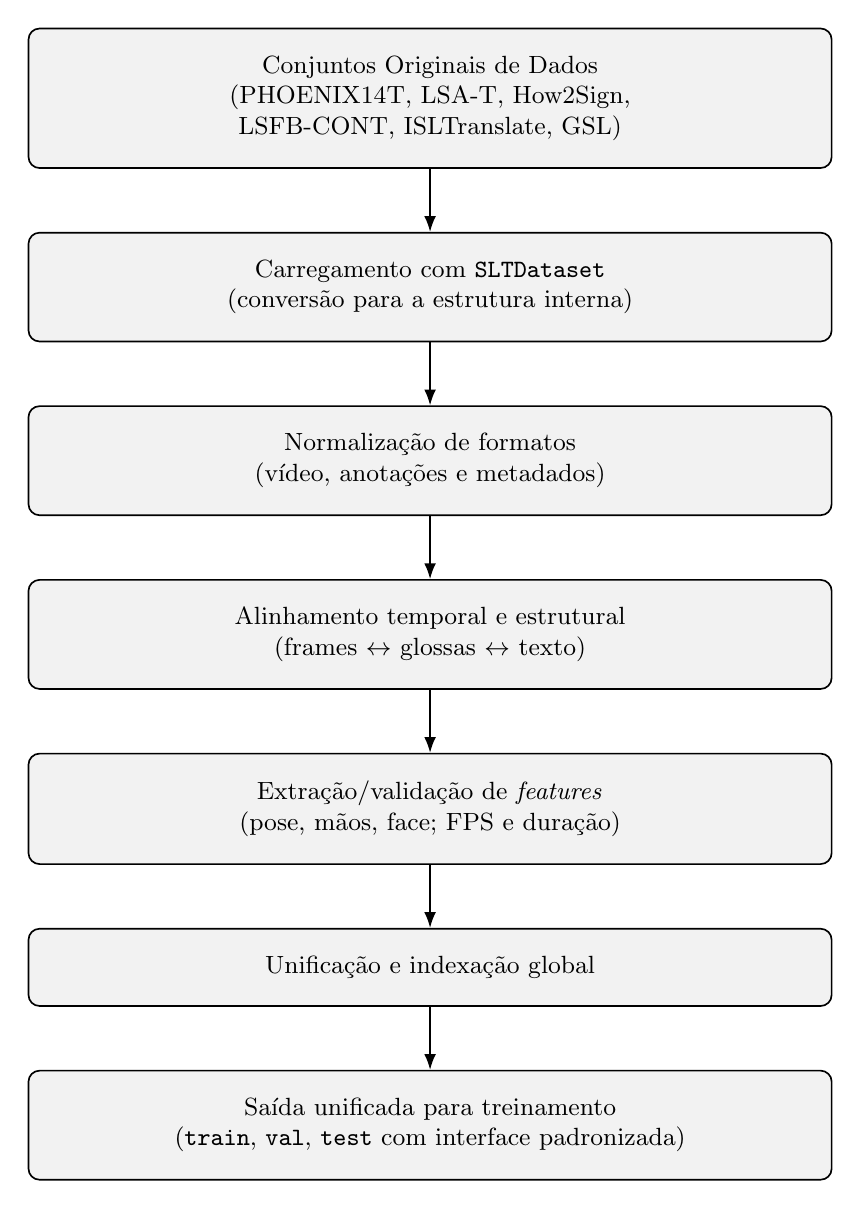
\begin{tikzpicture}[
  node distance=8mm,
  >=Latex,
  font=\small,
  box/.style={
    rectangle, rounded corners,
    draw=black, line width=0.6pt,
    fill=gray!10,
    inner sep=3.5mm,
    text width=9.5cm,
    align=center
  },
  arrow/.style={->, line width=0.6pt}
]

\node[box] (datasets) {Conjuntos Originais de Dados\\(PHOENIX14T, LSA-T, How2Sign, LSFB-CONT, ISLTranslate, GSL)};

\node[box, below=of datasets] (load) {Carregamento com \texttt{SLTDataset}\\(conversão para a estrutura interna)};

\node[box, below=of load] (norm) {Normalização de formatos\\(vídeo, anotações e metadados)};

\node[box, below=of norm] (align) {Alinhamento temporal e estrutural\\(frames $\leftrightarrow$ glossas $\leftrightarrow$ texto)};

\node[box, below=of align] (feat) {Extração/validação de \emph{features}\\(pose, mãos, face; FPS e duração)};

\node[box, below=of feat] (merge) {Unificação e indexação global};

\node[box, below=of merge] (out) {Saída unificada para treinamento\\(\texttt{train}, \texttt{val}, \texttt{test} com interface padronizada)};

\draw[arrow] (datasets) -- (load);
\draw[arrow] (load) -- (norm);
\draw[arrow] (norm) -- (align);
\draw[arrow] (align) -- (feat);
\draw[arrow] (feat) -- (merge);
\draw[arrow] (merge) -- (out);

\end{tikzpicture}
\caption{Fluxo de unificação dos dados com \texttt{slt\_datasets}.}
\label{fig:unificacao_slt_datasets}
\end{figure}

\section{Metodologia de Aumento de Dados com Base em Signformer}

\subsection{A Escolha Pelo \textit{Signformer}}
Do ponto de vista conceitual, o \textit{Signformer} parte do princípio de que a informação linguística crucial para a tradução em língua de sinais está codificada principalmente na cinemática de mãos, face e corpo, e não em texturas, cores ou fundo da cena \cite{Yang2024Signformer,Kim2022KeypointSLT}. Assim, a entrada do modelo é a sequência temporal de \emph{keypoints} normalizados extraídos do vídeo, o que comprime fortemente a dimensionalidade do problema e introduz invariâncias úteis (escala, translação e iluminação) \cite{Lugaresi2019MediaPipe,MediaPipeHolisticDocs}. Essa “desvisualização” do sinal reduz a variabilidade espúria entre bases e facilita treinar modelos portáveis com recursos computacionais moderados.

Sob a ótica de modelagem, o \textit{Signformer} se vale de autoatenção para capturar dependências de longo alcance na sequência de marcos, algo particularmente relevante em sinais contínuos, onde unidades semânticas se alongam no tempo e se sobrepõem (mãos + expressões faciais) \cite{Yang2024Signformer}. A atenção permite que o modelo integre pistas de diferentes janelas temporais sem impor um tamanho de contexto fixo, acomodando variações de velocidade de execução entre sinalizadores e efeitos de coarticulação típicos da modalidade gestual-visual.

Em termos de robustez a \textit{domain shift}, operar sobre \emph{keypoints} normalizados atenua diferenças de cenário, câmera e iluminação quando combinamos corpora heterogêneos. Na prática, essa escolha metodológica desloca a variância dominante do domínio visual (fundo/ruído) para o domínio articulatório (movimento e configuração), que é o que queremos que o modelo aprenda \cite{Kim2022KeypointSLT,DalBianco2022LSAT}. Ademais, mesmo após a consolidação dos conjuntos empregados, o volume total de dados permanece modesto para os padrões de modelos que processam vídeo cru, conforme discutido na literatura de SLT/SLR \cite{Camgoz2018NeuralSLT,Koller2020SurveySLR}.

Do ponto de vista operacional, o pipeline do \textit{Signformer} é direto:extração dos marcos por quadro \cite{Lugaresi2019MediaPipe,MediaPipeHolisticDocs},  normalização e padronização temporal para um comprimento alvo, e  alimentação da sequência resultante em um codificador Transformer \cite{Yang2024Signformer}. Como não há estágios de extração visual com CNN/ViT, simplifica-se a engenharia (menos pontos de falha, menos hiperparâmetros sensíveis) e libera-se memória para trabalhar com \emph{batch sizes} maiores, o que acelera a convergência e melhora a estabilidade do treinamento.

No treinamento supervisionado, o decodificador textual do \textit{Signformer} segue o regime padrão de \textit{teacher forcing} com entropia cruzada, o que facilita a adoção de práticas consolidadas de NMT (agendadores de taxa de aprendizado, \textit{label smoothing}, \textit{early stopping}) \cite{Yang2024Signformer}. Além disso, o decodificador aceita naturalmente múltiplas referências por amostra (original e variantes geradas por \textit{back-translation}/paráfrase), permitindo aprendizagem com diversidade superficial controlada sem qualquer alteração estrutural no modelo.

Outra vantagem prática é a interpretabilidade relativa: ao operar em marcos, torna-se possível inspecionar mapas de atenção ao longo do tempo e inferir quais regiões (mãos, face, tronco) ou quais intervalos temporais contribuíram mais para a predição \cite{Yang2024Signformer}, favorecendo análises de erro e ajustes finos no pré-processamento (por exemplo, reforçar a qualidade dos marcos de mão quando a atenção se concentra consistentemente naquele subespaço).

Como limitações, reconhece-se a dependência da qualidade da extração de \emph{keypoints}: oclusões, \textit{tracking} instável e desbalanceamentos de quadros podem degradar a representação \cite{Lugaresi2019MediaPipe,MediaPipeHolisticDocs}. Esses efeitos são mitigáveis com checagens de sanidade (proporção de marcos válidos por frame), suavização temporal leve, interpolação de lacunas curtas e \textit{augmentations} conservadores (ruído gaussiano pequeno nas mãos/face e \textit{time warping} suave). Ainda assim, dado que a quantidade de informação inclusa nas imagens, que é perdida quando se trabalha com pontos-chave, é muito grande, arquiteturas baseadas em vídeo cru podem levar vantagem, ao custo de bem mais dados e hardware.

\section{Aumento de Dados com Retrotradução, Paráfrases e Perturbações de Poses}
\label{sec:aumento-retro-parapose}

Nesta etapa investigamos se a combinação de retrotradução, geração de paráfrases e aumentos em sequências de \emph{keypoints} melhora a generalização entre línguas e reduz a esparsidade lexical (por exemplo, a taxa de \emph{singletons}) nos corpora unificados. O princípio é criar variantes textuais semanticamente equivalentes alinhadas à mesma janela de vídeo e, em paralelo, introduzir perturbações controladas nas poses que preservem a plausibilidade cinemática. Mantemos o mesmo pré-processamento de texto e vídeo descrito anteriormente em todo o conjunto; treinamos modelos com e sem aumento, reportando resultados \emph{in-domain}, \emph{cross-domain} e, quando aplicável, com \emph{signer-held-out}.

\subsection{Aumento textual por retrotradução e paráfrases com LLMs}
\label{subsec:retro-paraf-llm}

A retrotradução é um mecanismo consolidado em MT para aproveitar dados monolíngues: traduz-se a sentença de destino para um idioma pivô e, em seguida, traduz-se de volta para o idioma original, produzindo uma variante sintaticamente diferente porém equivalente em conteúdo \cite{Sennrich2016BT,Edunov2018BTScale}. Além disso, a própria técnica de retrotradução já foi explorada para gerar grandes conjuntos de paráfrases (como o ParaNMT) a partir de bitextos, mostrando ganhos em diversidade superficial e em tarefas a jusante \cite{Wieting2018ParaNMT}. Em SLT, há evidências de que incorporar dados sintéticos por caminhos análogos pode aliviar a escassez de paralelos \cite{Zhou2021SignBT}. Neste trabalho seguimos essas linhas, mas substituímos os sistemas de tradução dedicados por \emph{LLMs} comerciais de última geração para executar tanto a retrotradução quanto a paráfrase, em conformidade com tendências recentes de aumento de dados orientado por LLMs \cite{Ding2024LLMDA,ChatGPTDA2023,Oh2023LLMDA}.

Operacionalmente, partimos das sentenças-alvo já alinhadas a cada janela de vídeo e pedimos ao LLM para produzir duas famílias de variantes. A primeira família consiste em paráfrases no mesmo idioma de destino da amostra, controlando temperatura baixa e instruções explícitas de preservação de entidades, números, tempos e pronomes. A segunda família consiste em variantes obtidas por retrotradução com um \emph{pivot} predefinido. Adotamos uma política de pivôs que privilegia o inglês e o alemão como eixos de interdependência linguística: para sentenças cujo idioma de destino não seja inglês nem alemão, geramos duas retrotraduções independentes, uma via \textit{t}\,$\rightarrow$\,EN\,$\rightarrow$\,\textit{t} e outra via \textit{t}\,$\rightarrow$\,DE\,$\rightarrow$\,\textit{t}. Quando o idioma de destino já é inglês ou alemão, utilizamos o espanhol como pivô único, isto é, EN\,$\rightarrow$\,ES\,$\rightarrow$\,EN ou DE\,$\rightarrow$\,ES\,$\rightarrow$\,DE. Essa regra cria um acoplamento sistemático entre as línguas de maior cobertura (\emph{high-resource}) e as demais, o que nos permite testar explicitamente a hipótese de transferência: se a retrotradução induz uma interdependência útil entre distribuições, esperamos ganhos de generalização entre línguas e redução da esparsidade lexical medida sobre o manifesto unificado.

Para evitar deriva semântica, instruímos o LLM a não introduzir eventos ou negações ausentes e a manter o registro estilístico da fonte. Inspirados por achados de \emph{back-translation} em larga escala, variamos levemente o decodificador para promover diversidade controlada, análogo ao uso de amostragem/ruído observado como mais eficaz do que \emph{beams} estritos em muitos cenários \cite{Edunov2018BTScale}. Cada variante gerada permanece vinculada ao mesmo identificador da amostra e à mesma janela temporal do vídeo, preservando a segmentação e a comparabilidade com a referência original.

A validação automática das variantes textuais segue o \emph{modus operandi} adotado em trabalhos de geração/filtragem de dados sintéticos. Medimos similaridade semântica com \emph{sentence embeddings} (SBERT) e rejeitamos saídas abaixo de um limiar de cosseno, prática comum quando o objetivo é manter o significado proposicional \cite{Reimers2019SBERT}. Em paralelo, calculamos \textsc{chrF}/\textsc{chrF++} para controlar a distância superficial entre candidata e referência, uma métrica que tem melhor comportamento em línguas morfologicamente ricas \cite{Popovic2015chrF,WMT2017chrFpp}. Também reportamos \emph{BLEU} padronizado com \texttt{sacreBLEU}, garantindo reprodutibilidade e comparabilidade entre execuções e com a literatura \cite{Post2018SacreBLEU}. Como verificação semântica adicional, computamos \emph{BERTScore}, que tende a correlacionar melhor com julgamentos humanos em geração de sentenças \cite{Zhang2019BERTScore}. Esse conjunto de verificações nos permite rejeitar quase-cópias e variantes que alterem o conteúdo, algo igualmente recomendado em corpora de paráfrases gerados por retrotradução \cite{Wieting2018ParaNMT}. Por fim, aplicamos deduplicação por n-grama e \emph{minhash}, conservando apenas variantes que de fato aumentem a diversidade.

No regime de treinamento, avaliamos tanto a mistura direta de originais e sintéticos desde o início quanto um currículo em que os exemplos sintéticos entram apenas após algumas épocas de aquecimento. Mantemos a mesma normalização Unicode e os mesmos padrões de tokenização da etapa de unificação para evitar enviesar as métricas. Nossos resultados são estratificados por corpus e por língua, com ênfase em três indicadores: variação nas métricas de tradução (BLEU/\textsc{chrF}/\emph{BERTScore}), impacto em cenários \emph{cross-lingual} ao treinar com retrotraduções via EN/DE, e mudança na distribuição de frequência dos tipos (redução da taxa de \emph{singletons} e da cauda longa), que é calculada diretamente sobre o manifesto consolidado.

\subsection{Aumento em poses: perturbações plausíveis e checagens cinemáticas}
\label{subsec:aumento-poses}

As sequências de \emph{keypoints} recebem perturbações leves para fortalecer a robustez a variações de captura, oclusões e instabilidades de rastreamento. As transformações são aplicadas \emph{on-the-fly} e respeitam a coerência entre corpo, mãos e face, de modo que uma transformação rígida global permaneça consistente em todas as modalidades. Adotamos deslocamentos e escalas pequenas em coordenadas normalizadas, rotações moderadas no plano e variações temporais suaves por \emph{time-warping} e recorte com reamostragem, preservando o comprimento alvo. Para simular falhas de detecção frequentes em dedos e articulações distais, introduzimos \emph{keypoint dropout} com reconstrução por interpolação, seguindo a motivação de robustez a \emph{missing joints} observada em estudos de atividade humana baseada em esqueleto \cite{WACV2020KeypointDropout,Springer2021OcclusionDropout}. Complementarmente, exploramos mistura e composição de transformações em ablações, bem como ideias de \emph{auto-augmentation} de poses para elevar a diversidade sob restrições geométricas diferenciáveis, como apresentado em \emph{PoseAug} \cite{Gong2021PoseAug}. Em todos os casos, rejeitamos sequências cuja distribuição de comprimentos de ossos se afaste significativamente do original, condição suficiente para filtrar casos não plausíveis. Essa política aproxima-se do que relatam trabalhos recentes que visam generalização entre domínios com dados de esqueleto \cite{WACV2024RealisticSkelAug}.

% Eu sei que tá cagado
\begin{figure}[htbp]
\centering
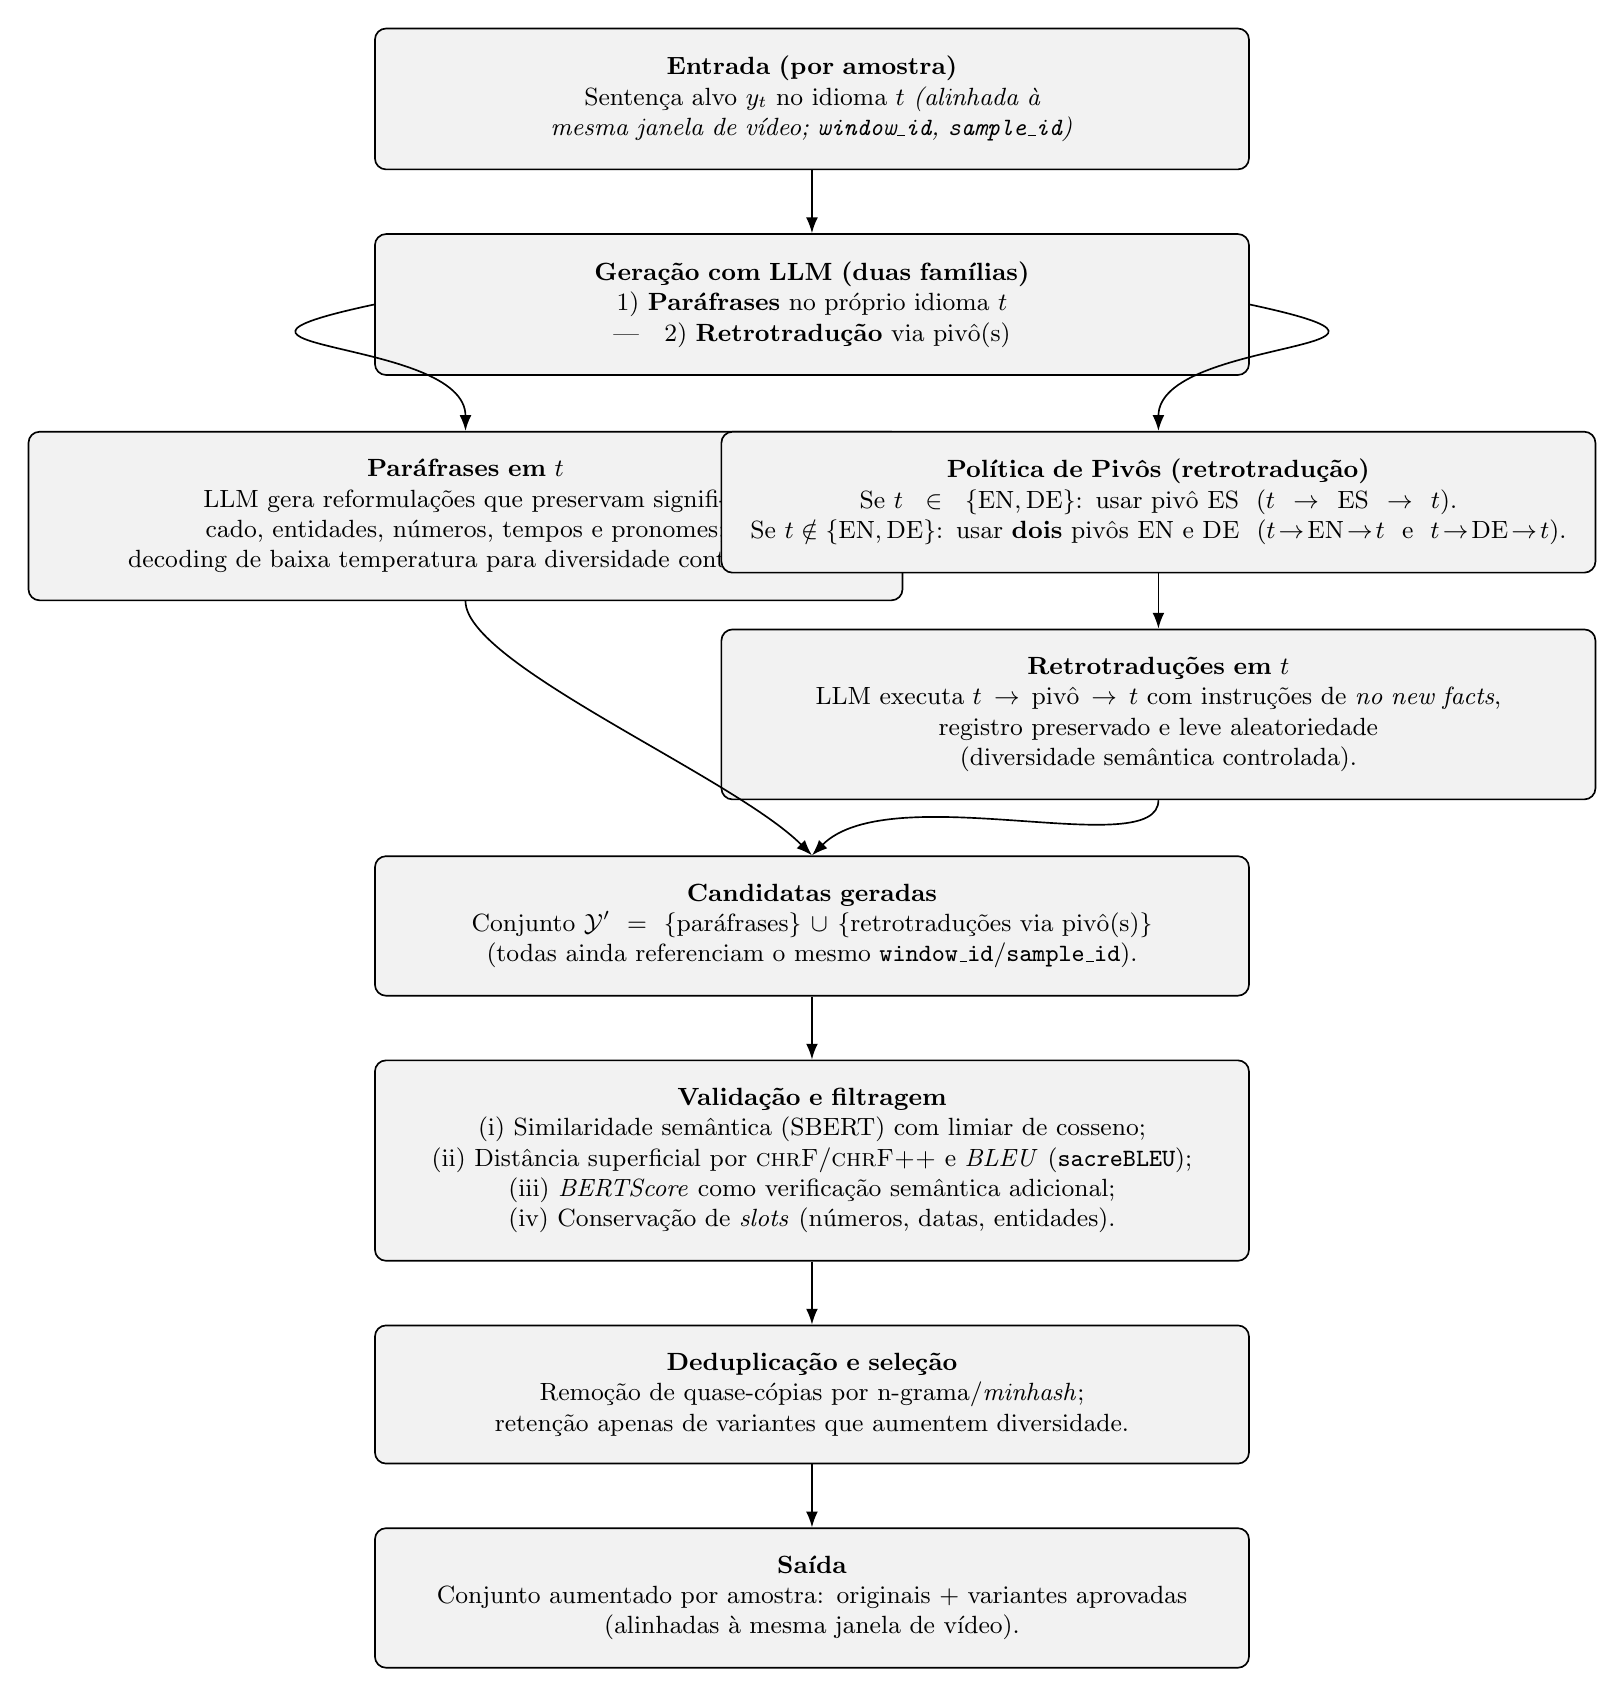
\begin{tikzpicture}[
  node distance=8mm,
  >=Latex,
  font=\small,
  box/.style={
    rectangle, rounded corners,
    draw=black, line width=0.6pt,
    fill=gray!10,
    inner sep=3.5mm,
    text width=10.4cm,
    align=center
  },
  arrow/.style={->, line width=0.6pt}
]

% Top nodes
\node[box] (input) {%
\textbf{Entrada (por amostra)}\\
Sentença alvo $y_t$ no idioma $t$ \emph{(alinhada à mesma janela de vídeo; \texttt{window\_id}, \texttt{sample\_id})}%
};

\node[box, below=of input] (split) {%
\textbf{Geração com LLM (duas famílias)}\\
1) \textbf{Paráfrases} no próprio idioma $t$ \quad|\quad
2) \textbf{Retrotradução} via pivô(s)%
};

% Branch A: Paraphrases (left)
\node[box, below=7mm of split, xshift=-44mm] (para) {%
\textbf{Paráfrases em $t$}\\
LLM gera reformulações que preservam significado, entidades, números, tempos e pronomes;\\
decoding de baixa temperatura para diversidade controlada.%
};

% Branch B: Pivot policy + BT (right)
\node[box, below=7mm of split, xshift=44mm] (policy) {%
\textbf{Política de Pivôs (retrotradução)}\\
Se $t\in\{\mathrm{EN},\mathrm{DE}\}$: usar pivô $\mathrm{ES}$ \ ($t\!\rightarrow\!\mathrm{ES}\!\rightarrow\!t$).\\
Se $t\notin\{\mathrm{EN},\mathrm{DE}\}$: usar \textbf{dois} pivôs $\mathrm{EN}$ e $\mathrm{DE}$ \ ($t\!\rightarrow\!\mathrm{EN}\!\rightarrow\!t$ \ e \ $t\!\rightarrow\!\mathrm{DE}\!\rightarrow\!t$).%
};

\node[box, below=7mm of policy] (bt) {%
\textbf{Retrotraduções em $t$}\\
LLM executa $t\!\rightarrow\!\text{pivô}\!\rightarrow\!t$ com instruções de \emph{no new facts},\\
registro preservado e leve aleatoriedade (diversidade semântica controlada).%
};

% Merge and rest of the pipeline
\node[box, below=7mm of bt, xshift=-44mm] (merge) {%
\textbf{Candidatas geradas}\\
Conjunto $\mathcal{Y}'=\{\text{paráfrases}\}\cup\{\text{retrotraduções via pivô(s)}\}$\\
(todas ainda referenciam o mesmo \texttt{window\_id}/\texttt{sample\_id}).%
};

\node[box, below=of merge] (filter) {%
\textbf{Validação e filtragem}\\
(i) Similaridade semântica (SBERT) com limiar de cosseno; \\
(ii) Distância superficial por \textsc{chrF}/\textsc{chrF++} e \emph{BLEU} (\texttt{sacreBLEU}); \\
(iii) \emph{BERTScore} como verificação semântica adicional; \\
(iv) Conservação de \emph{slots} (números, datas, entidades).%
};

\node[box, below=of filter] (dedup) {%
\textbf{Deduplicação e seleção}\\
Remoção de quase-cópias por n-grama/\emph{minhash}; retenção apenas de variantes que aumentem diversidade.%
};

\node[box, below=of dedup] (out) {%
\textbf{Saída}\\
Conjunto aumentado por amostra: originais $+$ variantes aprovadas\\
(alinhadas à mesma janela de vídeo).%
};

% Arrows
\draw[arrow] (input) -- (split);
\draw[arrow] (split.west) .. controls +(-2.8,-0.6) and +(0,1.2) .. (para.north);
\draw[arrow] (split.east) .. controls +(2.8,-0.6) and +(0,1.2) .. (policy.north);
\draw[arrow] (policy) -- (bt);
\draw[arrow] (para.south) .. controls +(0,-0.8) and +(-1,1.0) .. (merge.north);
\draw[arrow] (bt.south) .. controls +(0,-0.8) and +(1,1.0) .. (merge.north);
\draw[arrow] (merge) -- (filter);
\draw[arrow] (filter) -- (dedup);
\draw[arrow] (dedup) -- (out);

\end{tikzpicture}
\caption{Fluxo de geração por LLM de paráfrases e retrotraduções com política de pivôs (EN/DE; ES para casos em EN/DE), validação, deduplicação e acoplamento à mesma janela de vídeo.}
\label{fig:flow_bt_paraphrase}
\end{figure}



\chapter{Desenvolvimento}


\chapter{Conclusão}

% Bibliografia http://liinwww.ira.uka.de/bibliography/index.html um
% site que cataloga no formato bibtex a bibliografia em computacao
% \bibliography{nomedoarquivo.bib} (sem extensao)
% \bibliographystyle{formato.bst} (sem extensao)

\bibliographystyle{abnt}
\bibliography{bibliografia} 

\apendices
\chapter{Um Apêndice}

\end{document}

